\documentclass[11pt,a4paper]{article}
\usepackage[utf8]{inputenc}
\usepackage[spanish]{babel}	%Idioma
\usepackage{amsmath}
\usepackage{url}
\makeatletter
\makeatother
\usepackage{amsfonts}
\usepackage{amssymb}
\usepackage{graphicx} 	%Añadir imágenes
\usepackage{geometry}	%Ajustar márgenes
\usepackage[export]{adjustbox}[2011/08/13]
\usepackage{float}
\restylefloat{table}
\usepackage[hidelinks]{hyperref}
\usepackage{titling}
\graphicspath{}
\usepackage{multirow}
\usepackage{caption}
\usepackage{multicol}
\usepackage{array}
\usepackage{eurosym}


%Opciones de encabezado y pie de página:
\usepackage{fancyhdr}
\pagestyle{fancy}
\lhead{Grado en Ingeniería Informática}
\rhead{Manual de Usuario}
\lfoot{Sistemas Gráficos}
\cfoot{}
\rfoot{\thepage}
\renewcommand{\headrulewidth}{0.4pt}
\renewcommand{\footrulewidth}{0.4pt}

%Opciones de fuente:
\usepackage[utf8]{inputenc}
\usepackage[default]{sourcesanspro}
\usepackage{sourcecodepro}
\usepackage[T1]{fontenc}

\setlength{\parindent}{15pt}
\setlength{\headheight}{15pt}
\setlength{\voffset}{10mm}

% Custom colors
\usepackage{color}
\definecolor{deepblue}{rgb}{0,0,0.5}
\definecolor{deepred}{rgb}{0.6,0,0}
\definecolor{deepgreen}{rgb}{0,0.5,0}
\hypersetup{
    colorlinks=true,
    linkcolor=black,
    urlcolor=blue,
}

\usepackage{listings}

\begin{document}
\sloppy
\begin{titlepage}
  \centering
  
\includegraphics[width=0.7\textwidth]{logo.png}\par\vspace{1cm}
  {\scshape\large Sistemas Gráficos \par} \vspace{1cm}
  {\huge\bfseries Diseño e implementación de \\ un sistema gráfico \par}
  \vspace{0.4cm}
  {\large\bfseries ---Manual---\\}
  \vspace{0.6cm}
  {\large\itshape  Guillermo Sandoval Schmidt  \par} \vspace{1.00cm}
  Curso 2019-2020 \\
  \vfill

  % Bottom of the page
  {\large \today\par}
\end{titlepage}

\pagenumbering{gobble}
\pagenumbering{arabic}
\tableofcontents
\thispagestyle{empty}

\newpage

\section{Grupo de prácticas}
\begin{itemize}
    \item \textbf{Nombre de Alumno:} Guillermo Sandoval Schmidt
    \item \textbf{Nombre de la Aplicación:} Tetris
\end{itemize}

\section{Ejecución}

Para poder ejecutar la aplicación tendremos que situarnos en la carpeta \textit{P2} que debe contener las carpetas \textit{audio, fonts, img, libs} y \textit{tetris}. Una vez situados en esta carpeta, ejecutaremos en nuestro terminal el comando \textbf{python -m SimpleHTTPServer}, abriremos una pestaña de nuestro navegador y accederemos a la dirección \textit{http://localhost:8000/}.\\

Finalmente, haremos click en el enlace \textit{tetris/} y ya solo quedará disfrutar el juego.

\section{Controles principales}

\begin{multicols}{2}

Los controles principales son:

\begin{itemize}
    \item \textbf{Movimiento de la pieza:} se utilizan las teclas \textbf{IZQUIERDA}, \textbf{DERECHA} y \textbf{ABAJO} para mover la pieza en las correspondientes direcciones.
    \item \textbf{Rotación de la pieza:} se utilizan las teclas \textbf{Q} y \textbf{E} para girar la pieza hacia la izquierda y la derecha respectivamente.
    \item \textbf{Caída libre de la pieza:} se utiliza las tecla \textbf{W} para guardar la pieza actual, intercambiándola por la que tuviesemos guardada si ese fuese el caso.
    \item \textbf{Caída libre de la pieza:} se utiliza las tecla \textbf{SPACE} para forzar a la pieza a caer de golpe hasta el fondo del tablero.
\end{itemize}

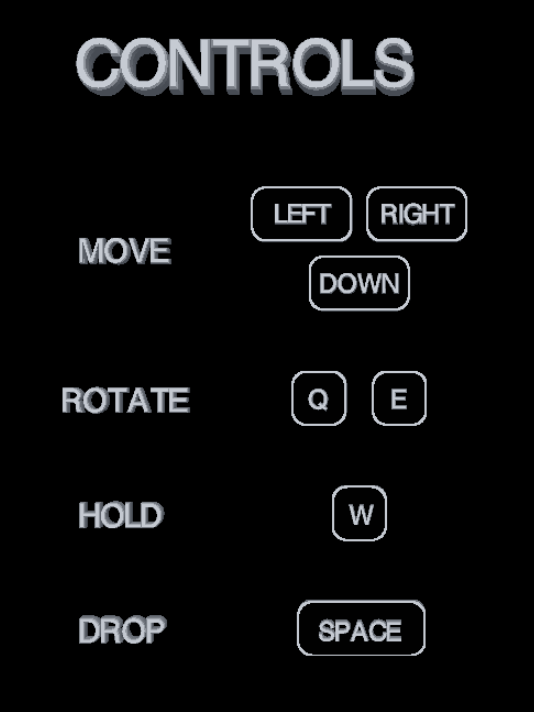
\includegraphics[scale=0.35]{controles.png}

\end{multicols}

\newpage

\section{Otros controles}
\subsection{Controles de cámara}

La aplicación cuenta con 4 cámaras, 1 libre y 3 fijas, entre las que se puede cambiar en cualquier momento utilizando las teclas numéricas del 1 al 4. Las cámaras son:

\begin{itemize}
    \item \textbf{Cámara 1 - Libre:} permite moverse libremente utilizando el ratón, con las siguientes funcionalidades:
    \begin{itemize}
        \item Click Izquierdo + arrastrar: controles orbitales.
        \item Click derecho + arrastrar: controles de posición.
        \item Rueda del ratón: control del zoom.
    \end{itemize}
    \item \textbf{Cámara 2 - Frontal:} permite observar la escena desde la parte frontal, es la cámara recomendada para jugar con mayor facilidad.
    \item \textbf{Cámara 3 - Lateral:} permite observar la escena desde el lateral derecho, es la cámara recomendada disfrutar del juego en 3D.
    \item \textbf{Cámara 4 . Inversa:} permite observar la escena desde como si estuviésemos boca abajo, es la cámara recomendada para aquellos que desean un reto a la hora de jugar, ya que los controles de se encuentran invertidos.
\end{itemize}

\subsection{Controles con ratón}

Además de los controles ya mencionados con el ratón para la cámara libre, la aplicación cuenta con un menú de inicio en el que podremos utilizar el ratón para pulsar el botón \textbf{PLAY} y dar comienzo a la partida.\\

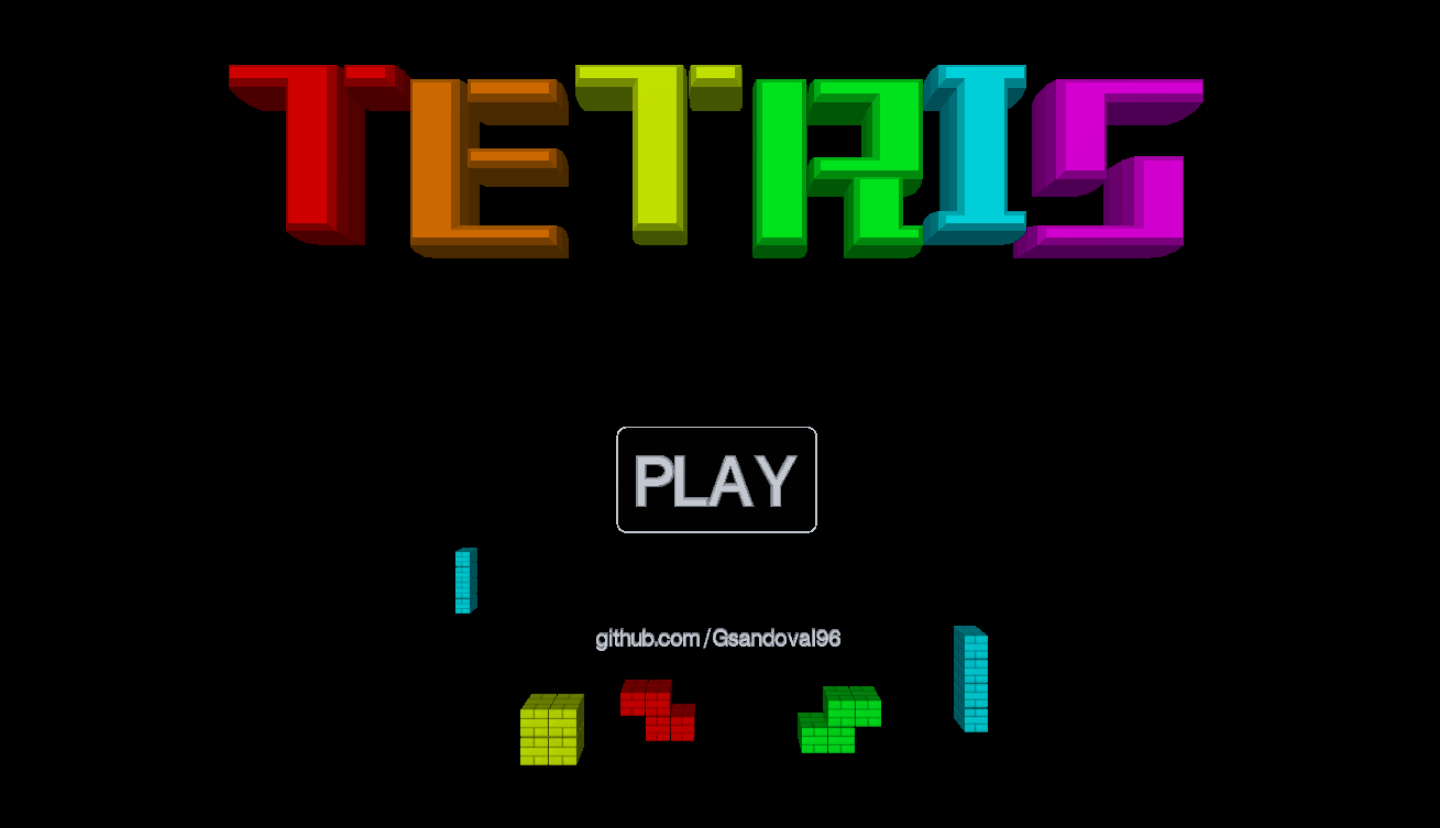
\includegraphics[scale=0.25]{menu.jpg}

\end{document}
